\chapter{初生对流检测系统的设计与实现}[Example]

\section{引言}[Number]
本章节设计并实现了一个对流初生检测的系统。此系统集成了前文章节中
所提及的对流初生检测算法模型,同时包括卫星原始数据的处理到对流检测的端到端处理过程。本章节将从
系统后端架构,系统任务计算模块和系统可视化模块三个部分展开。
\section{系统设计架构}
本文的系统采用的是前后端分离技术,B/S的设计架构,后端采用的是Flask的HTTP服务器,由Python
语言支持,前端是HTML、CSS、JavaScript编写的前端页面。运行方式为配置如表
~\ref{tab:env3}~内所示环境后,解压文件夹,命令行执行Run.sh。

\begin{table}[h]
	\renewcommand{\arraystretch}{1.3}
	\caption{系统运行环境}
	\label{tab:env3}
	\vspace{0.5em}\centering\wuhao
	\begin{tabular}{c c}
		\toprule[1.5pt] 环境参数 & 配置 \\
		\midrule[1pt] 
		系统环境 & Ubuntu/CentOs/RetHat \\
		软件环境 & tensorflow1.13.0、pytorch1.0.1、Anaconda3 \\
        硬件环境 & 内存1GB、显存1GB \\ 
		编程语言 & Python、HTML、CSS、JavaScript \\
		\bottomrule[1.5pt]
	\end{tabular}
\end{table}

本系统的后端为单任务流模式,
每当用户上传一个卫星云图数据文件,自动启动开启一个初生对流检测的执行,
由于卫星云图下存在很多个像素点,模型在执行过程中采用的是每个像素点周围的15$\times$15像元作为样本,
因此提取完像素后由系统自动判识并开启多进程执行该检测模型,
并将进度实时显示到前端的页面上,当所有像素点都判识完成,并完成结果合并成结果图,此时执行完成。

\section{检测执行模块设计}
此部分主要实现如何端到端的实现卫星云图的处理到对流初生检测过程。
本系统的综合架构如图~\ref{fig:system1}~所示。
此阶段依赖于用户对于检测上传的参数表达,检测上传包含卫星数据地址、模型选择以及执行模式等。
首先是卫星云图序列的处理,首先用户在上传任务之后,系统自动根据用户上传目录的卫星云图序列判断未检测的
数量,并将其添加到检测队列中。初生对流检测数据的处理则涉及到将提取多通道的卫星红外云图,以及利用
当前阈值法对其进行规则处理。此时如果采取的是多进程的执行模式,
检测执行模块会自动开启多进程执行,但是相应占用的系统资源也会增加。模型选择则是每次执行初生对流检测所采取的模型。

\begin{figure}[h]
	\centering
	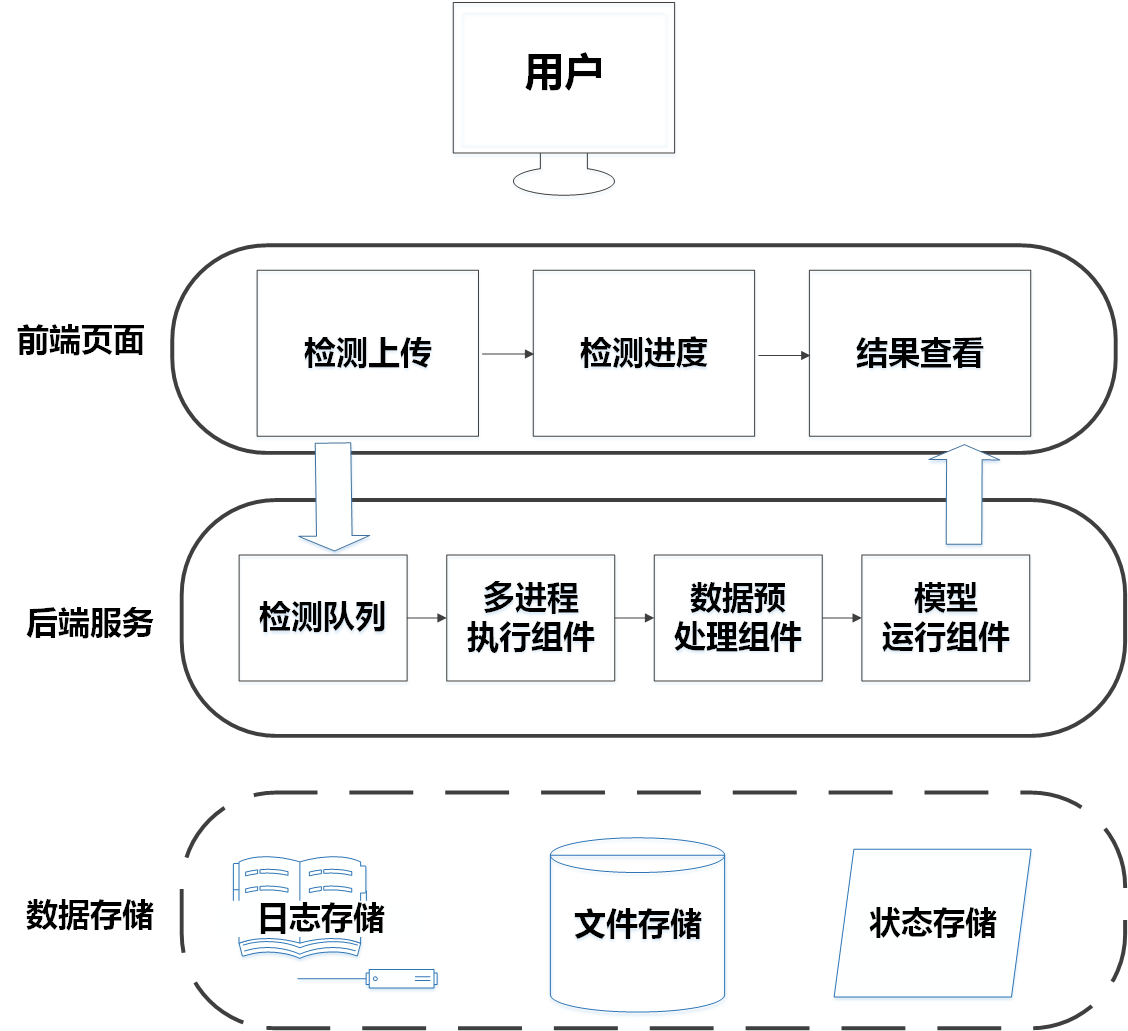
\includegraphics[width = 0.6\textwidth]{系统模块.png}
	\caption{系统综合架构}
	\label{fig:system1}
\end{figure}

同时系统还有错误检测和恢复的功能,如图~\ref{fig:err}~所示。
系统错误恢复是指系统执行过程中如果出现其他中断,例如断电、宕机等问题,
如果磁盘没有损坏则能够对检测进度进行恢复;错误检测则是如果存在例如时序不全或者卫星云图损坏等
错误,会自动检测而不是崩溃影响后续任务的执行进度。

\begin{figure}[h]
	\centering
	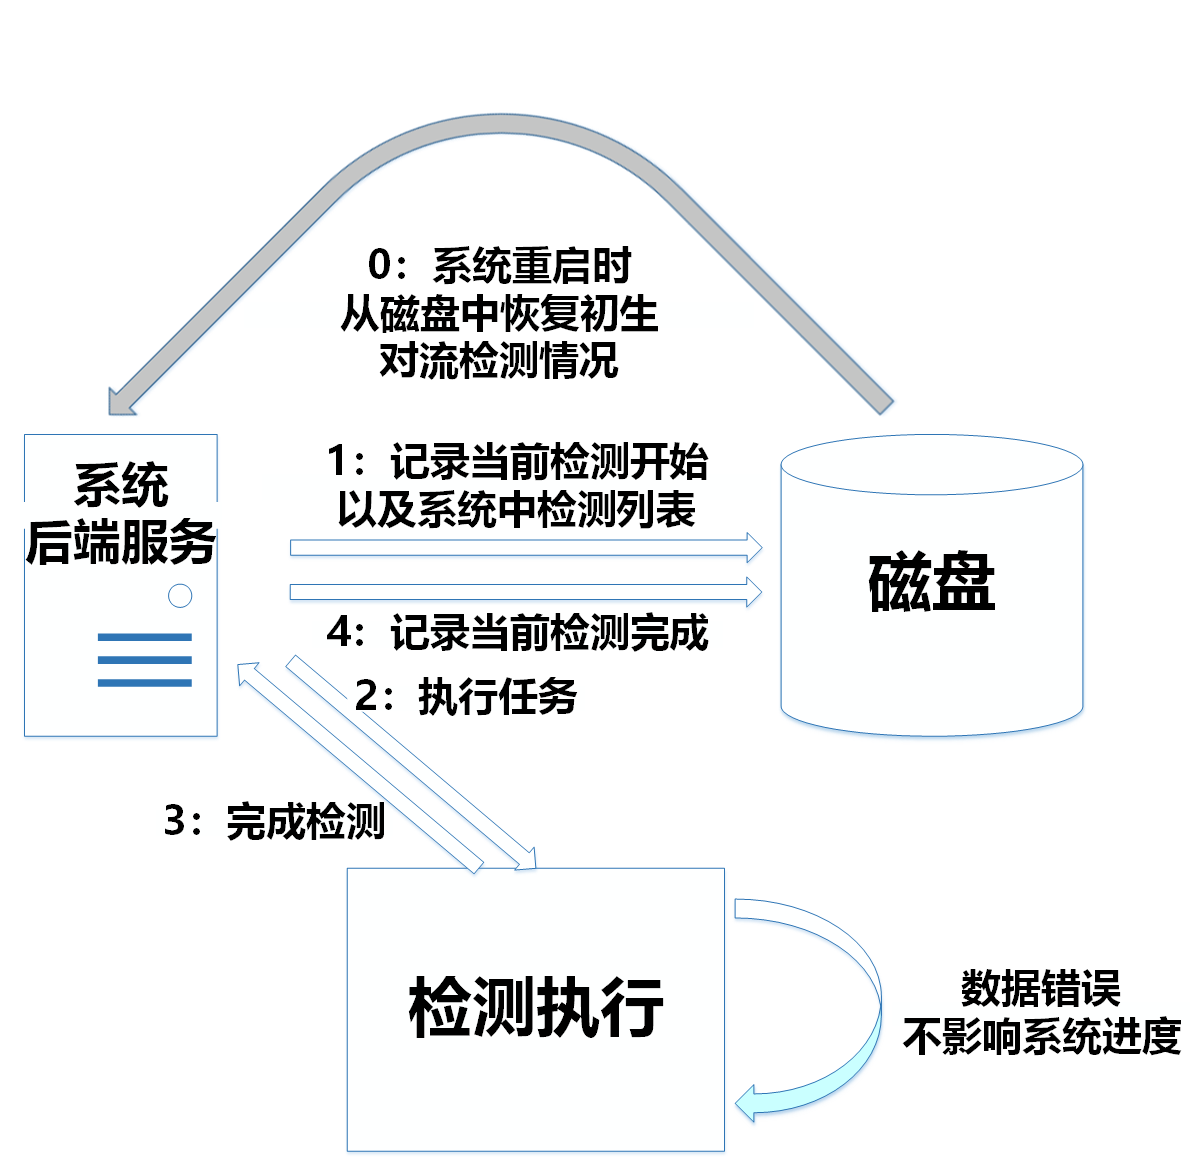
\includegraphics[width = 0.6\textwidth]{纠错模块.png}
	\caption{系统错误检测及恢复模块}
	\label{fig:err}
\end{figure}

\section{系统的可视化页面设计}
系统启动方式为在服务器运行脚本run.sh,启动后可通过主机地址加端口号(ip:port)的方式访问。
系统访问默认进入对流初生检测系统的可视化主界面,如图~\ref{fig:sys-main}~所示,主界面左侧有快捷访问的菜单栏。
可通过访问不同快捷菜单进入不同的系统界面。菜单栏中主界面为系统启动的默认界面同时具有查看检测进度的功能,
查看完成任务可查看历史检测结果,
任务上传负责上传检测任务,文件管理可直接以文件的形式查看检测数据。
\begin{figure}[h]
	\centering
	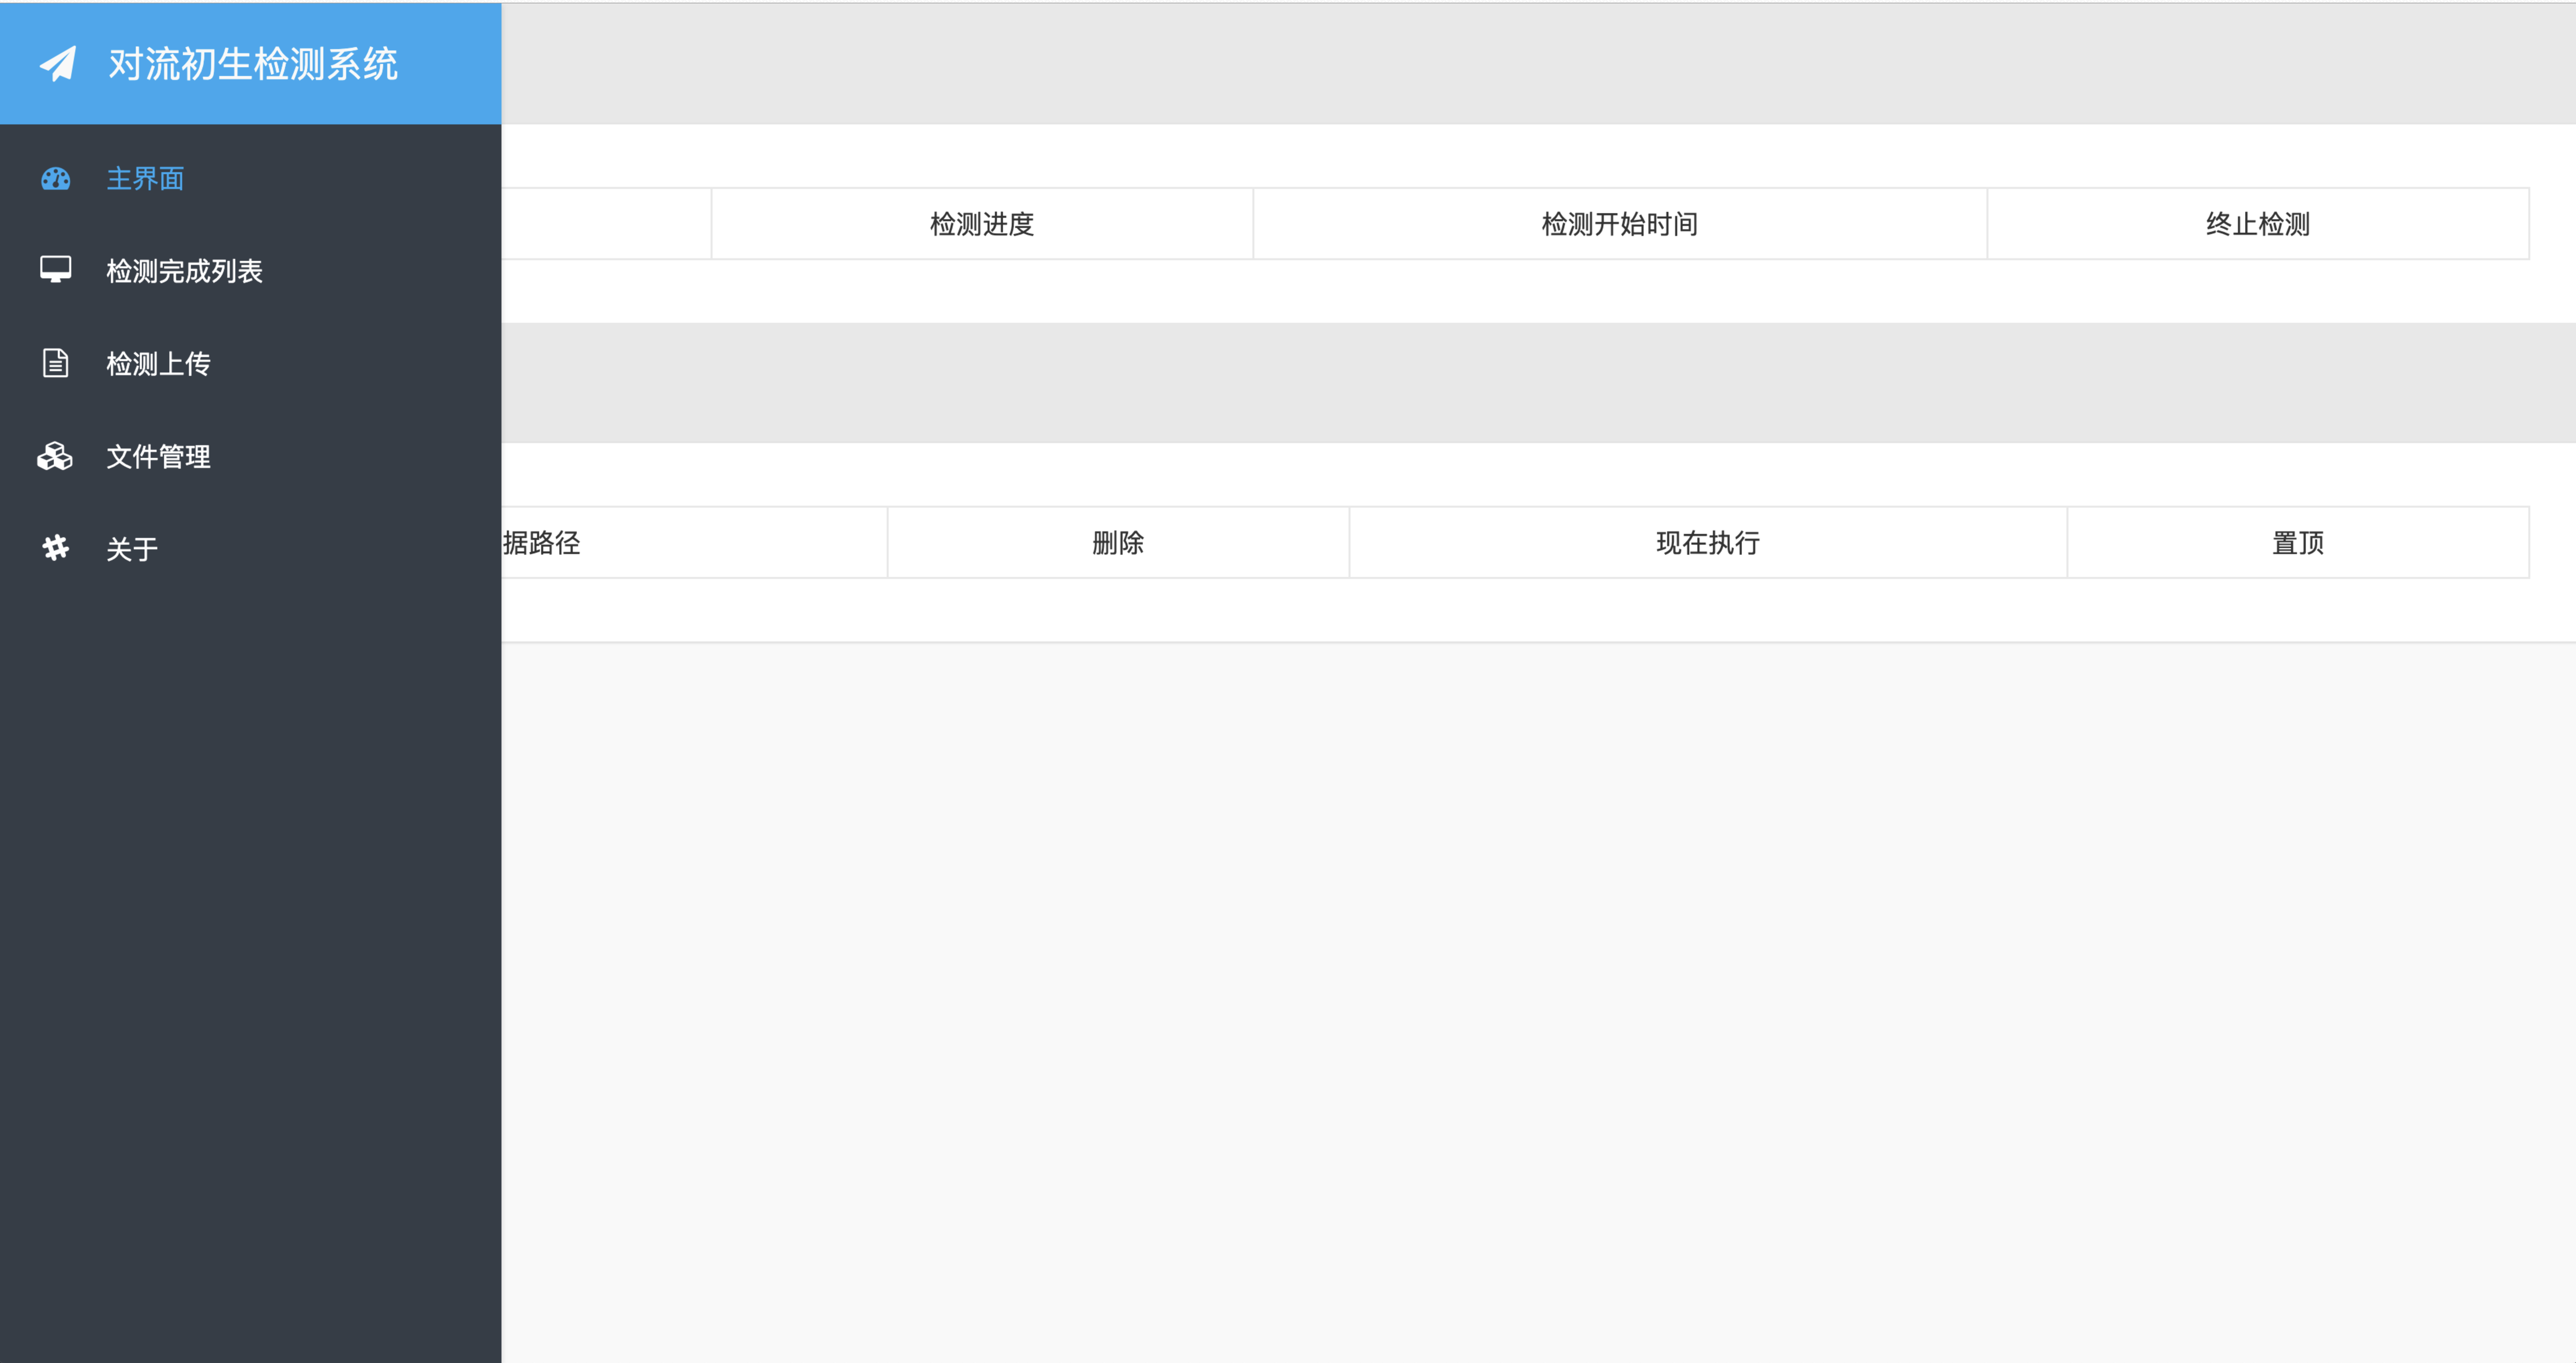
\includegraphics[width = 0.8\textwidth]{主界面2.png}
	\caption{系统默认界面及菜单栏}
	\label{fig:sys-main}
\end{figure}

\subsection{检测上传界面}
检测上传界面依次有任务目录,模型选择以及执行模式三个选项。
如果检测上传成功则会跳转至进度界面,
如果检测上传失败(例如目录不存在,模型不存在等)则会有弹窗提醒检测上传失败。
通常情况下检测上传的流程为先获取检测数据路径,以路径名作为任务名输入,可利用系统中的
文件管理可以获取到数据路径,其中的卫星数据按照日期由
新到旧排序,如图~\ref{fig:sys-getpath}~所示。
\begin{figure}[h]
	\centering
	\includegraphics[width = 0.8\textwidth]{获取路径2.png}
	\caption{文件管理界面获取路径}
	\label{fig:sys-getpath}
\end{figure}

之后进入检测上传界面输入路径,执行模式以及模型选择,如图~\ref{fig:sys-missupload}~所示。执行模式为1时会立即执行该任务,无需进入等待列表等待。
模型默认为本文的基准线模型Dense-S-RCNN,也可以采用其他模型进行预测。
\begin{figure}[h]
	\centering
	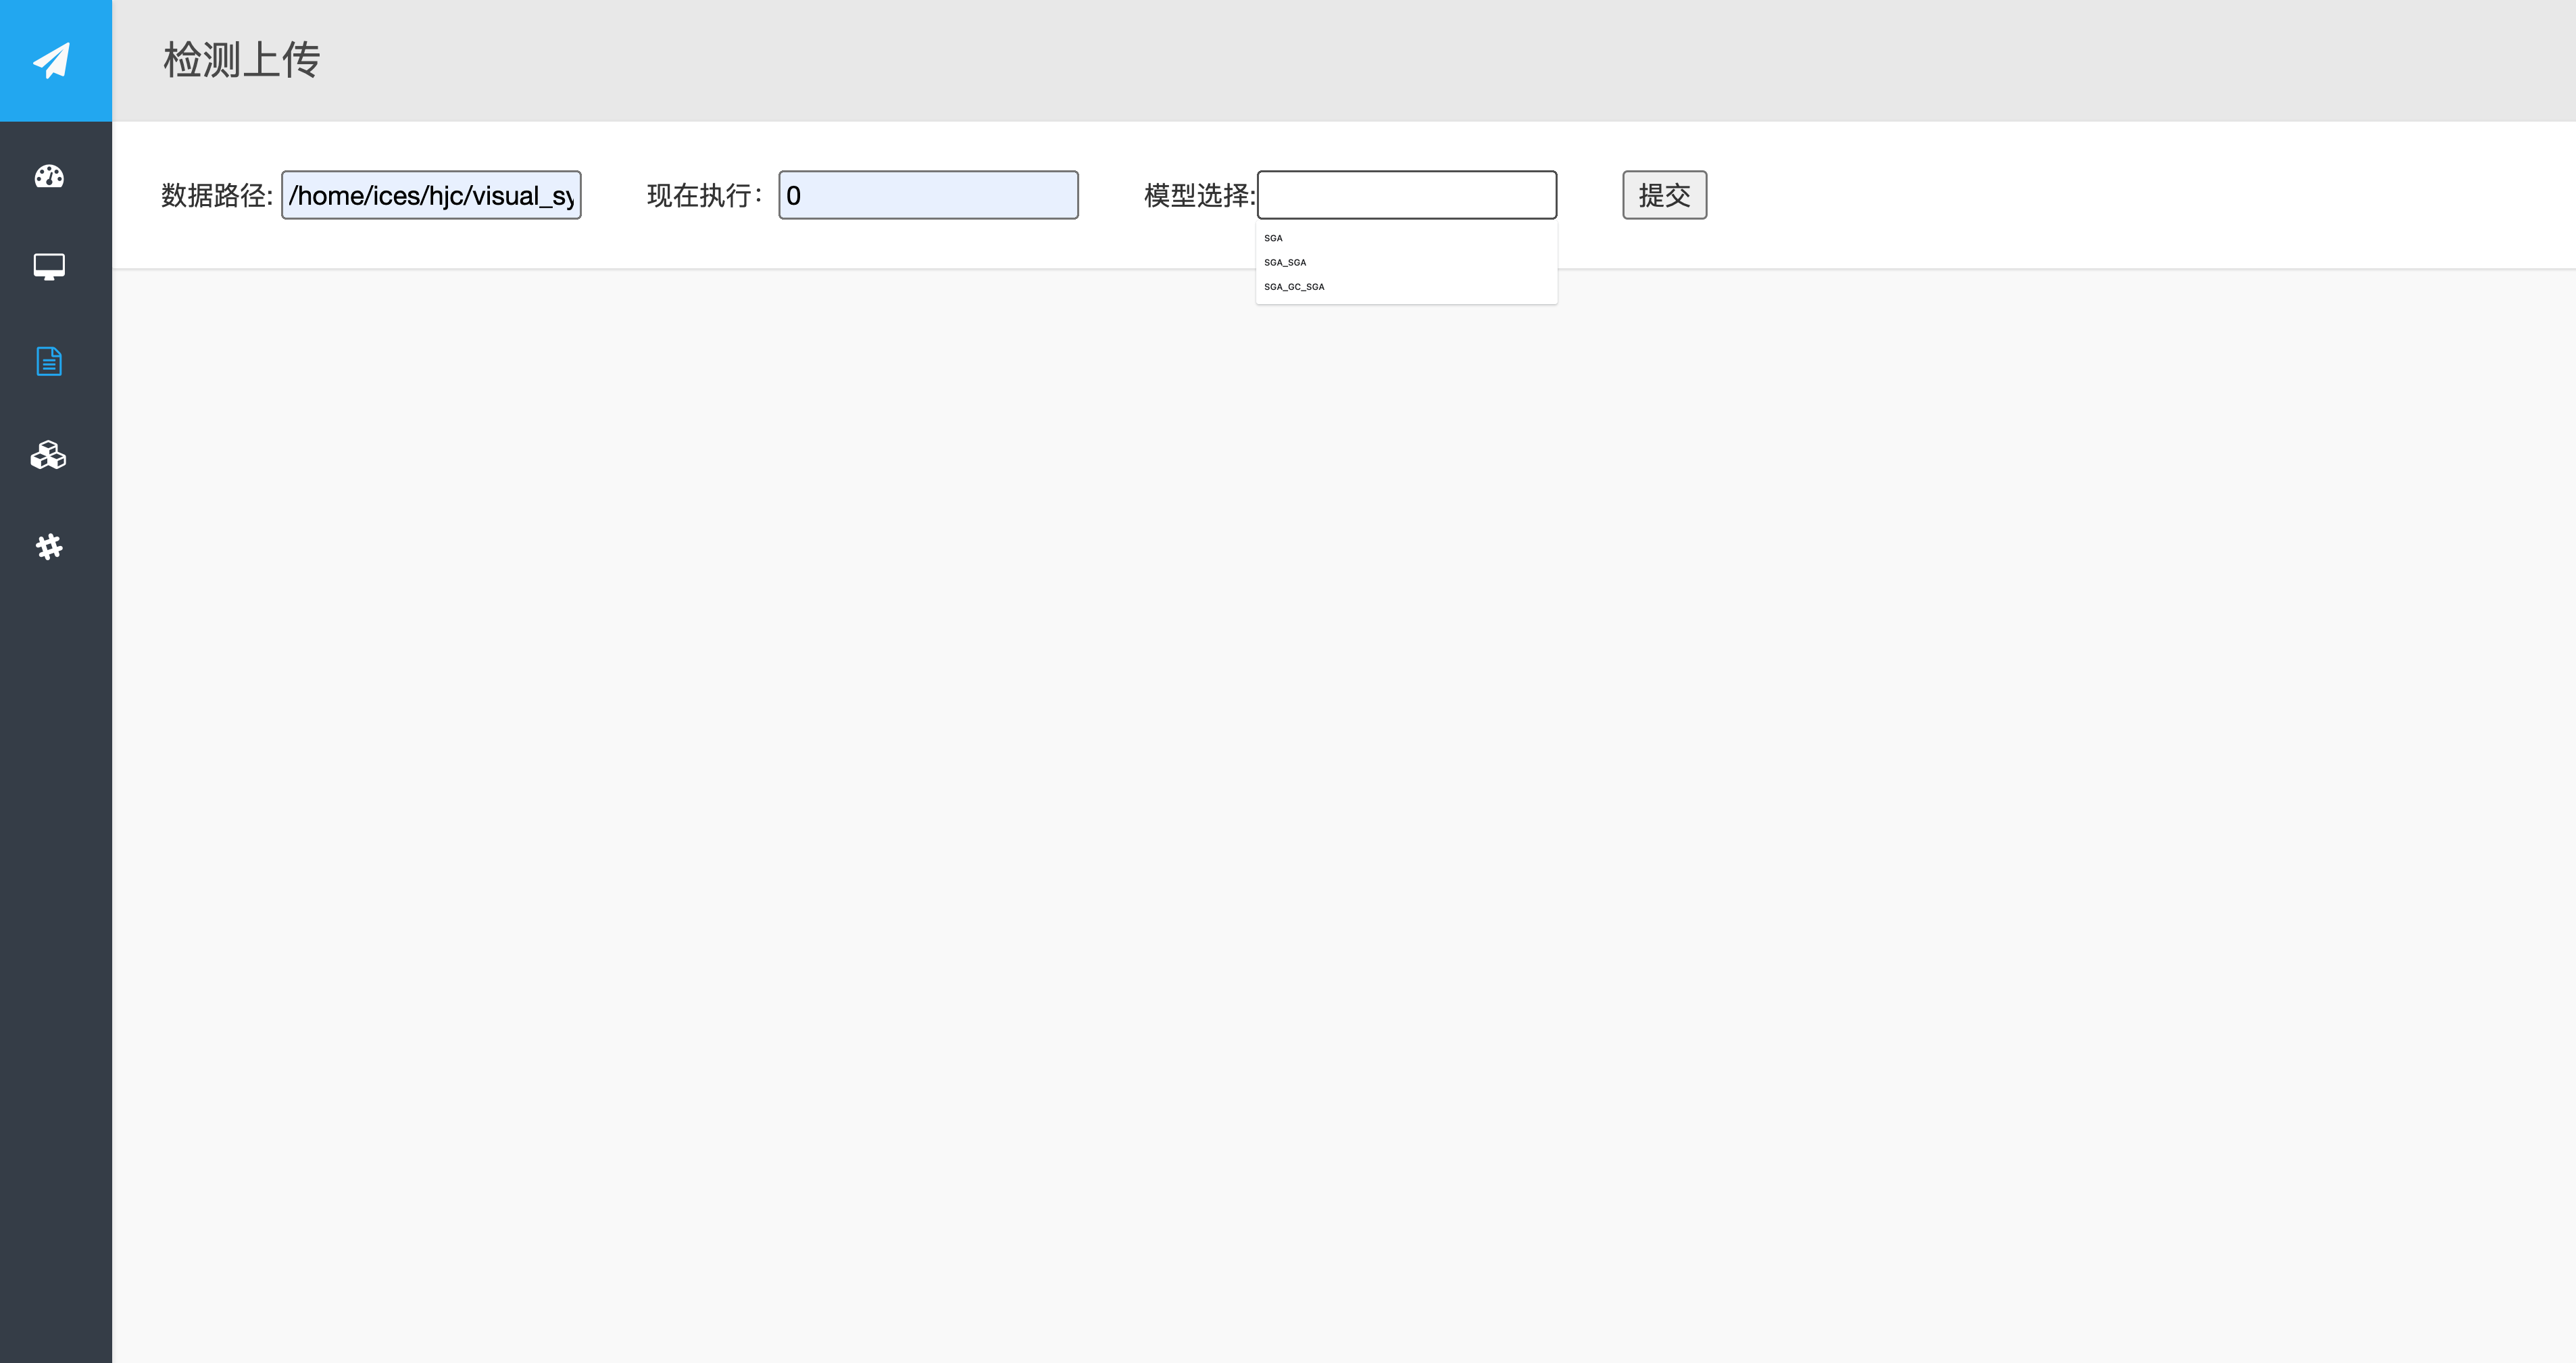
\includegraphics[width = 0.8\textwidth]{检测上传2.png}
	\caption{检测上传界面}
	\label{fig:sys-missupload}
\end{figure}

\subsection{检测进度界面}
此界面为检测的进度页面,如图~\ref{fig:sys-missjd}~所示,其中执行中的检测进度采用了ajax技术定时访问后端状态,从而实时显示到前端。
检测进度界面中在等待中的检测会按照排序
排队等待,用户也可以手动拖拽以调整其次序。如果用户选择终止程序,可以选择终止执行中的检测
。用户如果想直接执行后续等待中的检测,也可以选择立即执行,此时会有弹窗提醒,
如果选择否则无事发生,选择是则会中断执行中任务,立即执行等待中的检测。被中断的检测也会
排序在等待中检测的第一位。同时用户也可选择删除检测,此时会将等待中的检测删除。
\begin{figure}[h]
	\centering
	\includegraphics[width = 0.8\textwidth]{检测进度2.png}
	\caption{检测进度界面}
	\label{fig:sys-missjd}
\end{figure}

检测结束后,可通过查看检测完成列表来查看检测情况,如图~\ref{fig:sys-missdone}~所示,通常情况检测状态为完成(done),存在
一些情况会导致检测失败,比如数据长度不足或者模型不存在等,检测失败的情况不会影响后续数据的检测
进度。
\begin{figure}[h]
	\centering
	\includegraphics[width = 0.8\textwidth]{检测完成2.png}
	\caption{检测完成列表界面}
	\label{fig:sys-missdone}
\end{figure}

\subsection{结果预览界面}
检测执行完成后,会将数据输出结果重新输出到源数据文件夹下面,用户可以通过结果预览界面
查看检测结果文件是否正确输出出来。如图~\ref{fig:sys-1}~\ref{fig:sys-2}~\ref{fig:vis-ans}~所示。
\begin{figure}[h]
	\centering
	\includegraphics[width = 0.8\textwidth]{系统12.png}
	\caption{不同模型结果预览界面}
	\label{fig:sys-1}
\end{figure}

\begin{figure}[h]
	\centering
	\includegraphics[width = 0.8\textwidth]{系统22.png}
	\caption{模型输出结果预览界面}
	\label{fig:sys-2}
\end{figure}

\begin{figure}[h]
	\centering
	\subfigure[结果预览1]{
		\begin{minipage}[t]{0.4\linewidth}
			\centering
			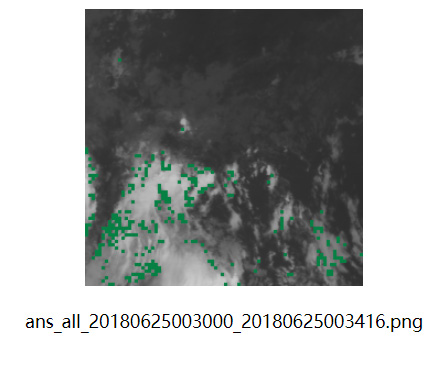
\includegraphics[width = 2.2in]{结果1.jpg}
		\end{minipage}
	}
	\subfigure[结果预览2]{
		\begin{minipage}[t]{0.4\linewidth}
			\centering
			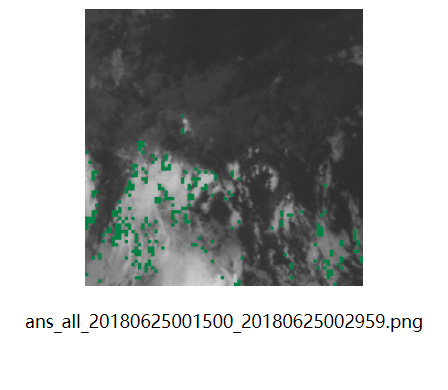
\includegraphics[width = 2.2in]{结果2.jpg}
		\end{minipage}
	}
	\caption{可视化模型运行结果图}
	\label{fig:vis-ans}
\end{figure}


\section{总结}
本章设计并实现了端到端的对流初生检测的系统。从系统的设计架构出发,
分为前后端以及存储三个模块。用户操作前端模块,可以上传卫星数据、终止检测以及查看检测结果。后端
主要代表系统的整个逻辑层,逻辑层中可多进程处理卫星数据预处理以及模型的运行等。存储部分负责
系统的稳定性,任务模块的变动会先写入磁盘,而后改变逻辑层状态,保证了系统的可恢复性。

\begin{figure}[h]
	\centering
	\subfigure[S-RCNN模型框架]{
		\begin{minipage}[t]{0.4\linewidth}
			\centering
			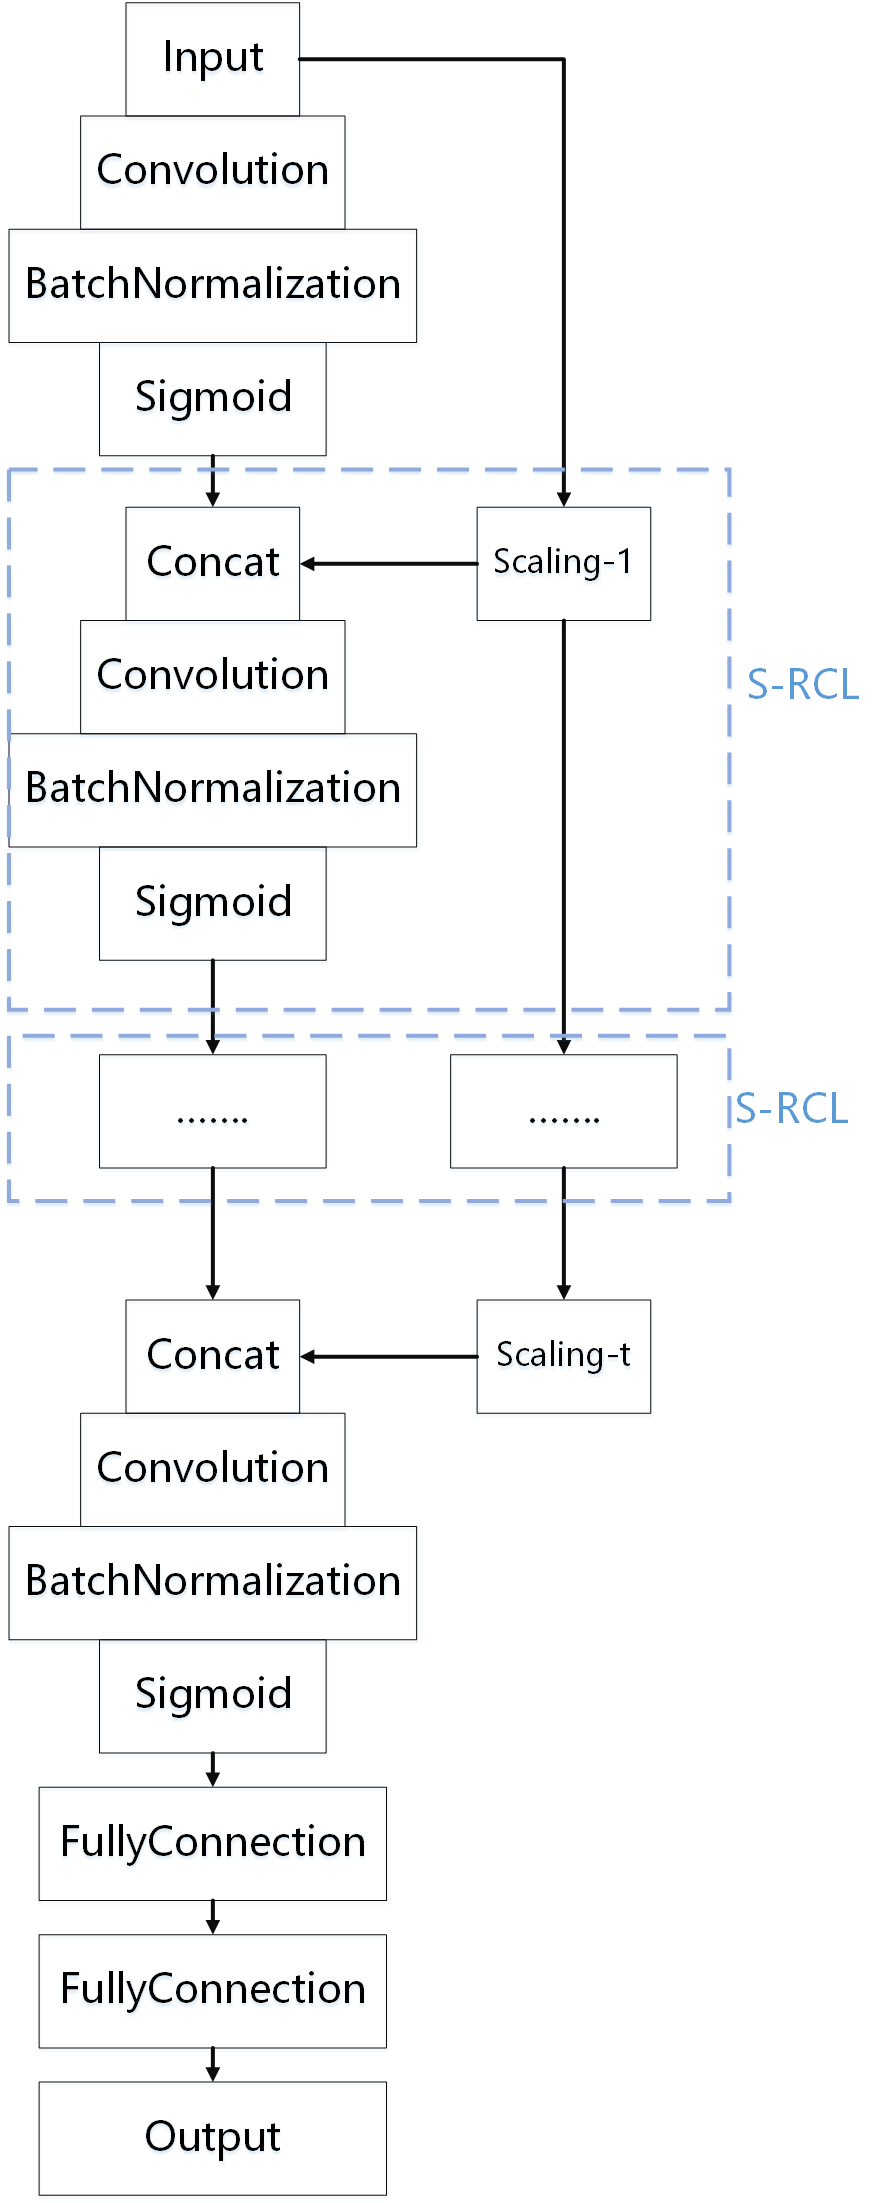
\includegraphics[width = 2in]{RCNN模型框架.png}
		\end{minipage}
	}
	\subfigure[Dense-S-RCNN连接结构]{
		\begin{minipage}[t]{0.4\linewidth}
			\centering
			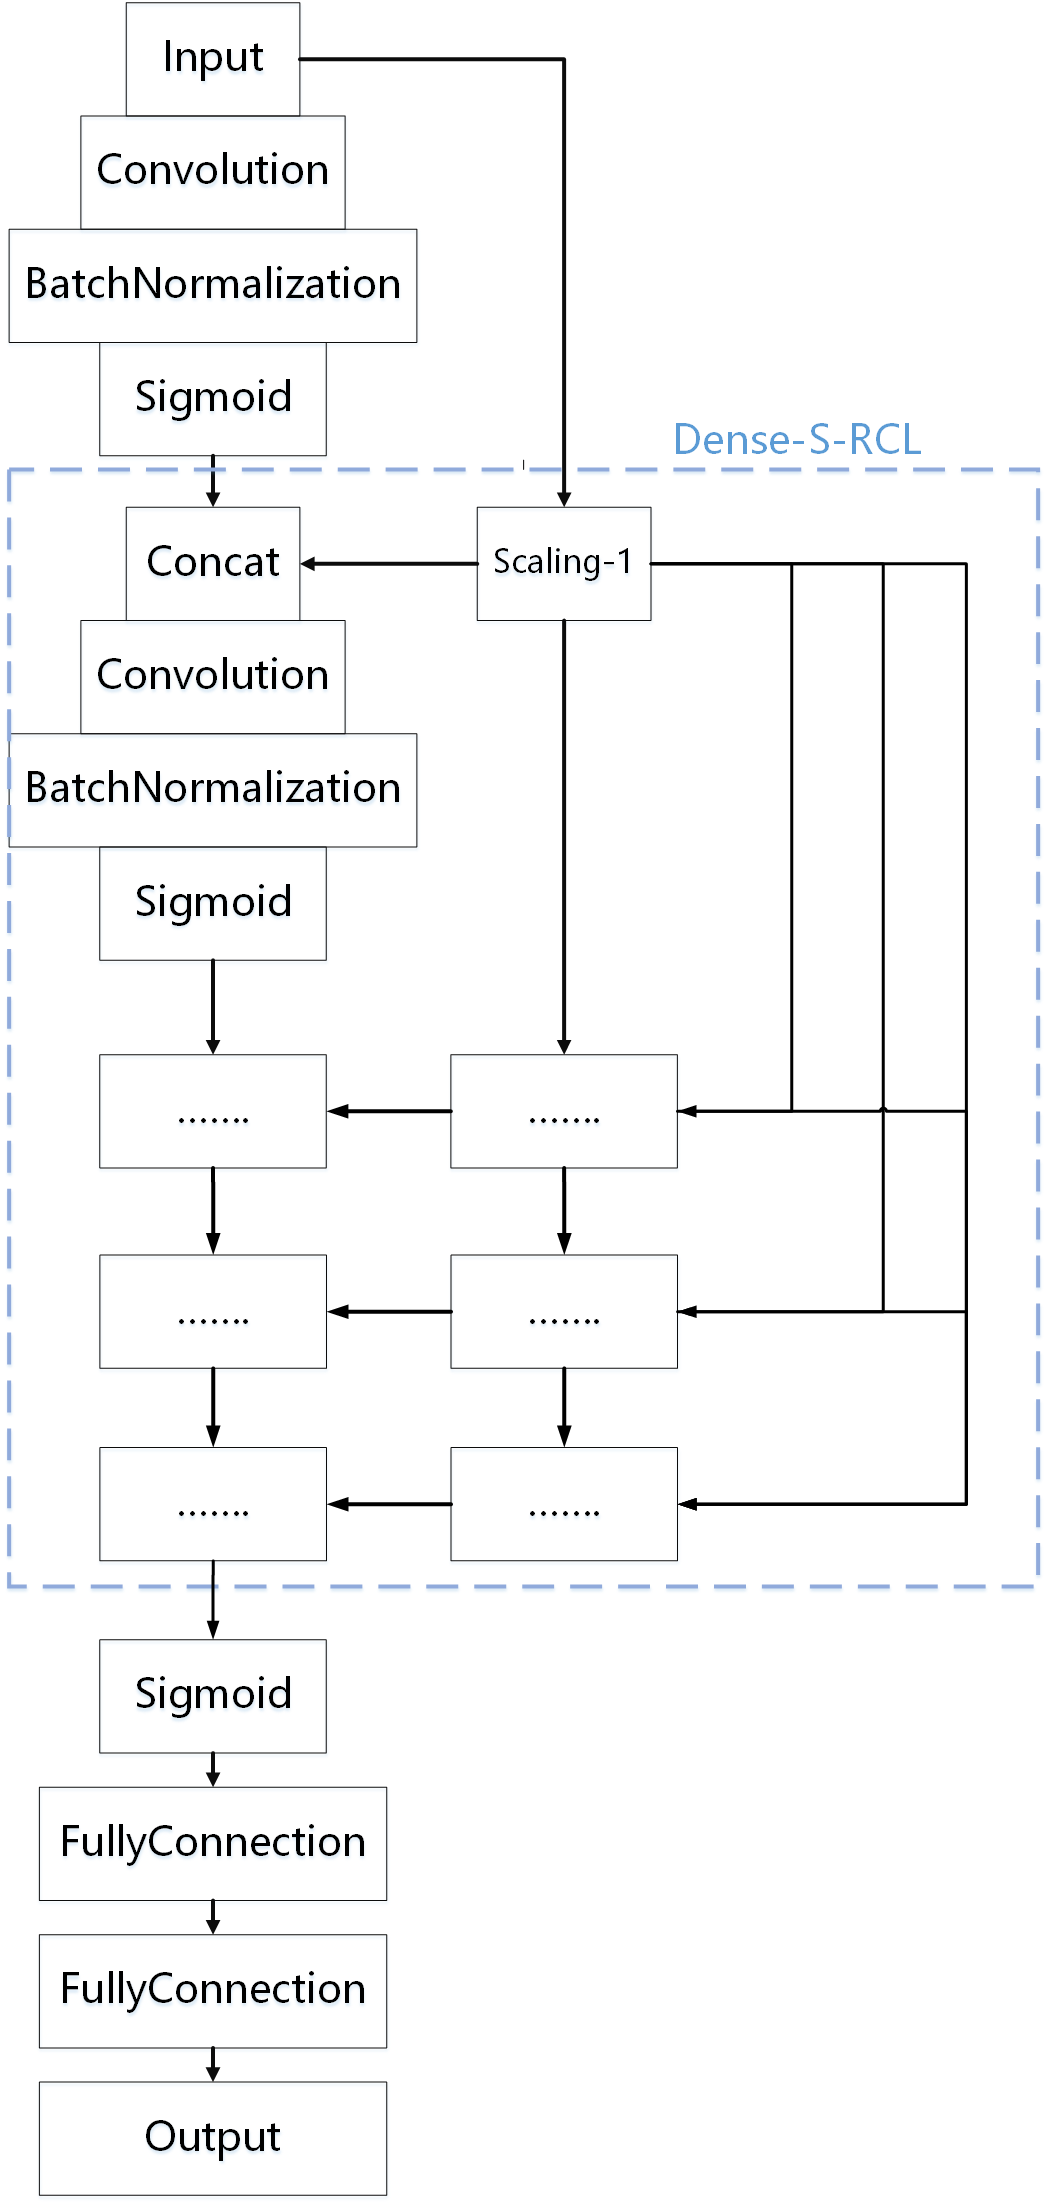
\includegraphics[width = 2.5in]{block.png}
		\end{minipage}
	}
	\caption{基于密集连接的多尺度特征金字塔对流初生检测模型架构}
	\label{RCNN_model}
\end{figure}
